Für die Umsetzung wurden handelsübliche Funksteckdosen verwendet, da diese relativ günstig in den meisten Geschäften zu haben sind. Diese erfüllen jedoch Standardmäßig einen anderen Zweck, diese werden über eine Fernbedienung ein bzw. aus geschaltet. Da es uns nicht möglich ist, Steckdosen mit dem Raspberry über Funk zu steuern, musste eine andere Möglichkeit her.\\
Uns kam die Idee, dass in diesen Steckdosen eigentlich nur ein Relais vorhanden sein muss, welches die 230V schaltet. Diese Tatsache machten wir uns zu nutze und suchten auf der Platine nach diesem Schaltpunkt und entwickelten eine passende Schaltung, welche diese Relais schaltet.\\
Um widerrechtliches steuern der Steckdosen durch gefinkelte Schüler zu verhindern und da das Funkmodul nur auf die Platine aufgelötet war, bauten wir diese Platine aus. Somit ist es nicht mehr möglich die Steckdosen mit der passenden Fernbedienung zu steuern.\\\\
Die Schaltung der Steckdose ist in keinster weise irgendwo dokumentiert, auch die auf der Schaltung vorhandenen IC's sind kaum bis gar nicht dokumentiert, weshalb es uns nicht möglich war die Funktionsweise der einzelnen Teile heraus zu finden. Durch Analysen der Leiterbahnen konnten wir uns eine grobe Übersicht über die Schaltung, zumindest soweit, dass wir den Hochspannungsteil und den Niederspannungsteil und das Relais finden konnten. Dieser Überblick reichte jedoch nicht aus, um den Schaltpunk des Relais zu finden. Der eigentliche Schaltpin am Relais konnte identifiziert werden, jedoch schaltet dieses Relais nur bei 48V, welche nicht möglich war anzulegen, deshalb musste eine andere Möglichkeit gefunden werden.\\ 
Die Art des Suchens war nicht sehr Sehenswert, denn wir versuchten mit anlegen einer Spannung abwechselnd an die Pins der IC's den Pin zu finden welcher das Relais schaltet. Nach kurzer Zeit war auch schon ein Punkt gefunden, dieser Punkt war jedoch nicht optimal, da dieser einen sehr hohen Strom zog, wenn diese Spannung angelegt wurde. Deshalb gingen wir von diesem Punkt aus und suchten einen besseren Punkt, diesen fanden wir. Hier wurde kein Nennenswerter Strom benötigt. Wir fanden außerdem heraus, dass das Anlegen an diesen Punkt von 5V genügt und diese Spannung von der Funkplatine verwendet werden konnte. Da anfangs der Strom an diesem Punkt auch sehr hoch war, beschlossen wir uns einen nicht gebrauchten IC zu entfernen, nach dem Entfernen dieses IC's ist der Strom deutlich gesunken.\\
Für die leichte Montage wurden die Vorhandenen Löcher, von der ursprünglichen Montage des Funkmoduls, verwendet. Über die Löcher wurde die Platine versorgt, diese Möglichkeit verwendeten auch wir, weshalb wir von dem gefundenen Punkt eine Drahtbrücke zum Loch machten. Die 5V waren sowieso schon auf einem der Löcher vorhanden. Um die ursprüngliche Funktion des Loches ab zu schalten trennten wir durch Entfernung eines Widerstandes die Leiterbahn auf. Nun musste nur mehr die Platine in die Löcher gesteckt werden. Die nötigen Signale sind bei den Löchern angelegt und werden über die Verbindung auf der Platine bereitgestellt.\\
Nun musste noch eine Lösung gefunden werden, wie mit dem Raspberry diese 2 Punkte verbunden werden konnten. Dies wurde mit einer Transistorschaltung realisiert. Wenn der Raspberry an einem der GPIO-Pins digital 1 (analog 3,3V DC) anlegt, so schaltet der Transistor und verbindet somit die zwei Punkte. \\
Dies war jedoch nicht genug, da noch eine Potentialtrennung zwischen Raspberry und Steckdose  notwendig war, wie ein Test ohne Potentialtrennung zeigt. (Siehe Punkt???). Diese lösten wir mit einem Optokoppler, welcher den Raspberry von der Steckdose trennen soll. Dies erfolgte mit der Schaltung ordnungsgemäß. Jedoch packten wir die Potentialtrennung auf den Header, welcher auf den Raspberry aufgesteckt wird, dies stellte sich als fataler Fehler heraus. (siehe Punkt ????)\\
Der finale Aufbau war dann wie folgt:\\
Auf die GPIO-Pins (siehe \autoref{fig:report_hardware_gpio1}) wird eine Platine(Header) gesteckt, welche die Transistorschaltung beinhaltet. Die Transistorschaltung schaltet die 5V Versorgung über einen Vorwiderstand den Optokoppler, welcher auf einer Platine in der Steckdose liegt. Die Verbindung wurde mit einem 2 poligen Draht, welcher auf beiden Seiten eine 3,5mm Mono Stecker montiert hat. Auf der Platine in der Steckdose ist nur der Optokoppler, der das Ein- bzw. Ausschalten der Steckdose vornimmt.\\
Für die Kommunikation mit dem Raspberry wird der GPIO Pin 7 verwendet. Die 5V Spannung und die Masse für das Schalten des Optokopplers wird der Pin 2(5V) und der Pin 6(0V) des Raspberrrys verwendet. Wichtig: Hier ist anzumerken, dass die Rasperrys Revision 1 und Revision 2 verschiedene Anordnung haben. Unsere Schaltung ist für Revision 2 entwickelt, es ist also nicht zu empfehlen, die Platine auf einem Revision 1 Raspberry zu verwenden, da er Schaden nehmen könnte.
\\
\begin{figure}[H]
\centering
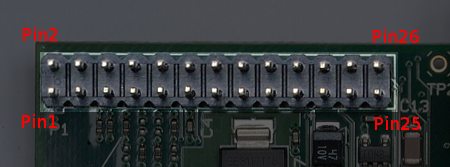
\includegraphics[keepaspectratio=true, width=10cm]{images/rpi/picPins.png}
\caption[GPIO-Pins]{GPIO-Pins\\ \textbf{Quelle:} http://elinux.org/Rpi\_Low-level\_peripherals}
\label{fig:report_hardware_gpio1}
% source: http://elinux.org/Rpi_Low-level_peripherals#General_Purpose_Input.2FOutput_.28GPIO.29
\end{figure}
\begin{figure}[H]
\centering
\rule{1cm}{1cm}
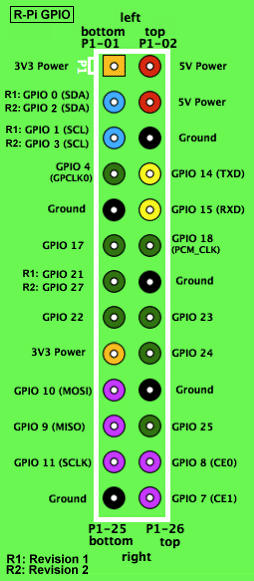
\includegraphics[keepaspectratio=true, width=7cm]{images/rpi/gpio.png}
% source: http://elinux.org/Rpi_Low-level_peripherals#General_Purpose_Input.2FOutput_.28GPIO.29
\caption[GPIO-Pinbelegung]{GPIO-Pinbelegung\\ \textbf{Quelle:}
\label{fig:report_hardware_gpio2} http://elinux.org/Rpi\_Low-level\_peripherals}
\end{figure}